\section{ADC}

The \href{http://www.analog.com/media/en/technical-documentation/data-sheets/229321fa.pdf}{LTC2292}
is a 40MHz, 12-bit differential input ADC. The schematic for this device is shown in
Figure~\ref{fig:ltc2292-schematic}. We use this device instead of the built-in FPGA ADCs
because those sample at a rate of 1Msps, which is insufficient for our needs. The difference signal
received by the ADC and passed to the FPGA has a frequency in the range of kHz to a few MHz, for a
which a 40MHz sampling rate is significantly more than the Nyquist frequency. The received signal
is received on two antennas, which allows for the angle of the received signal to be computed. These
are amplified, mixed and then amplified again before feeding into the ADC. By connecting the CLKA,
CLKB, and MUX pins together, we multiplex both channels together through the same output pins,
D01-D11A. The timing for this multiplexed output is shown in
Figure~\ref{fig:ltc2292-multiplex}. Table~\ref{tab:ltc2292-pinout} contains a list of all the ADC
pins and their connections.

\begin{figure}[h]
  \centering
  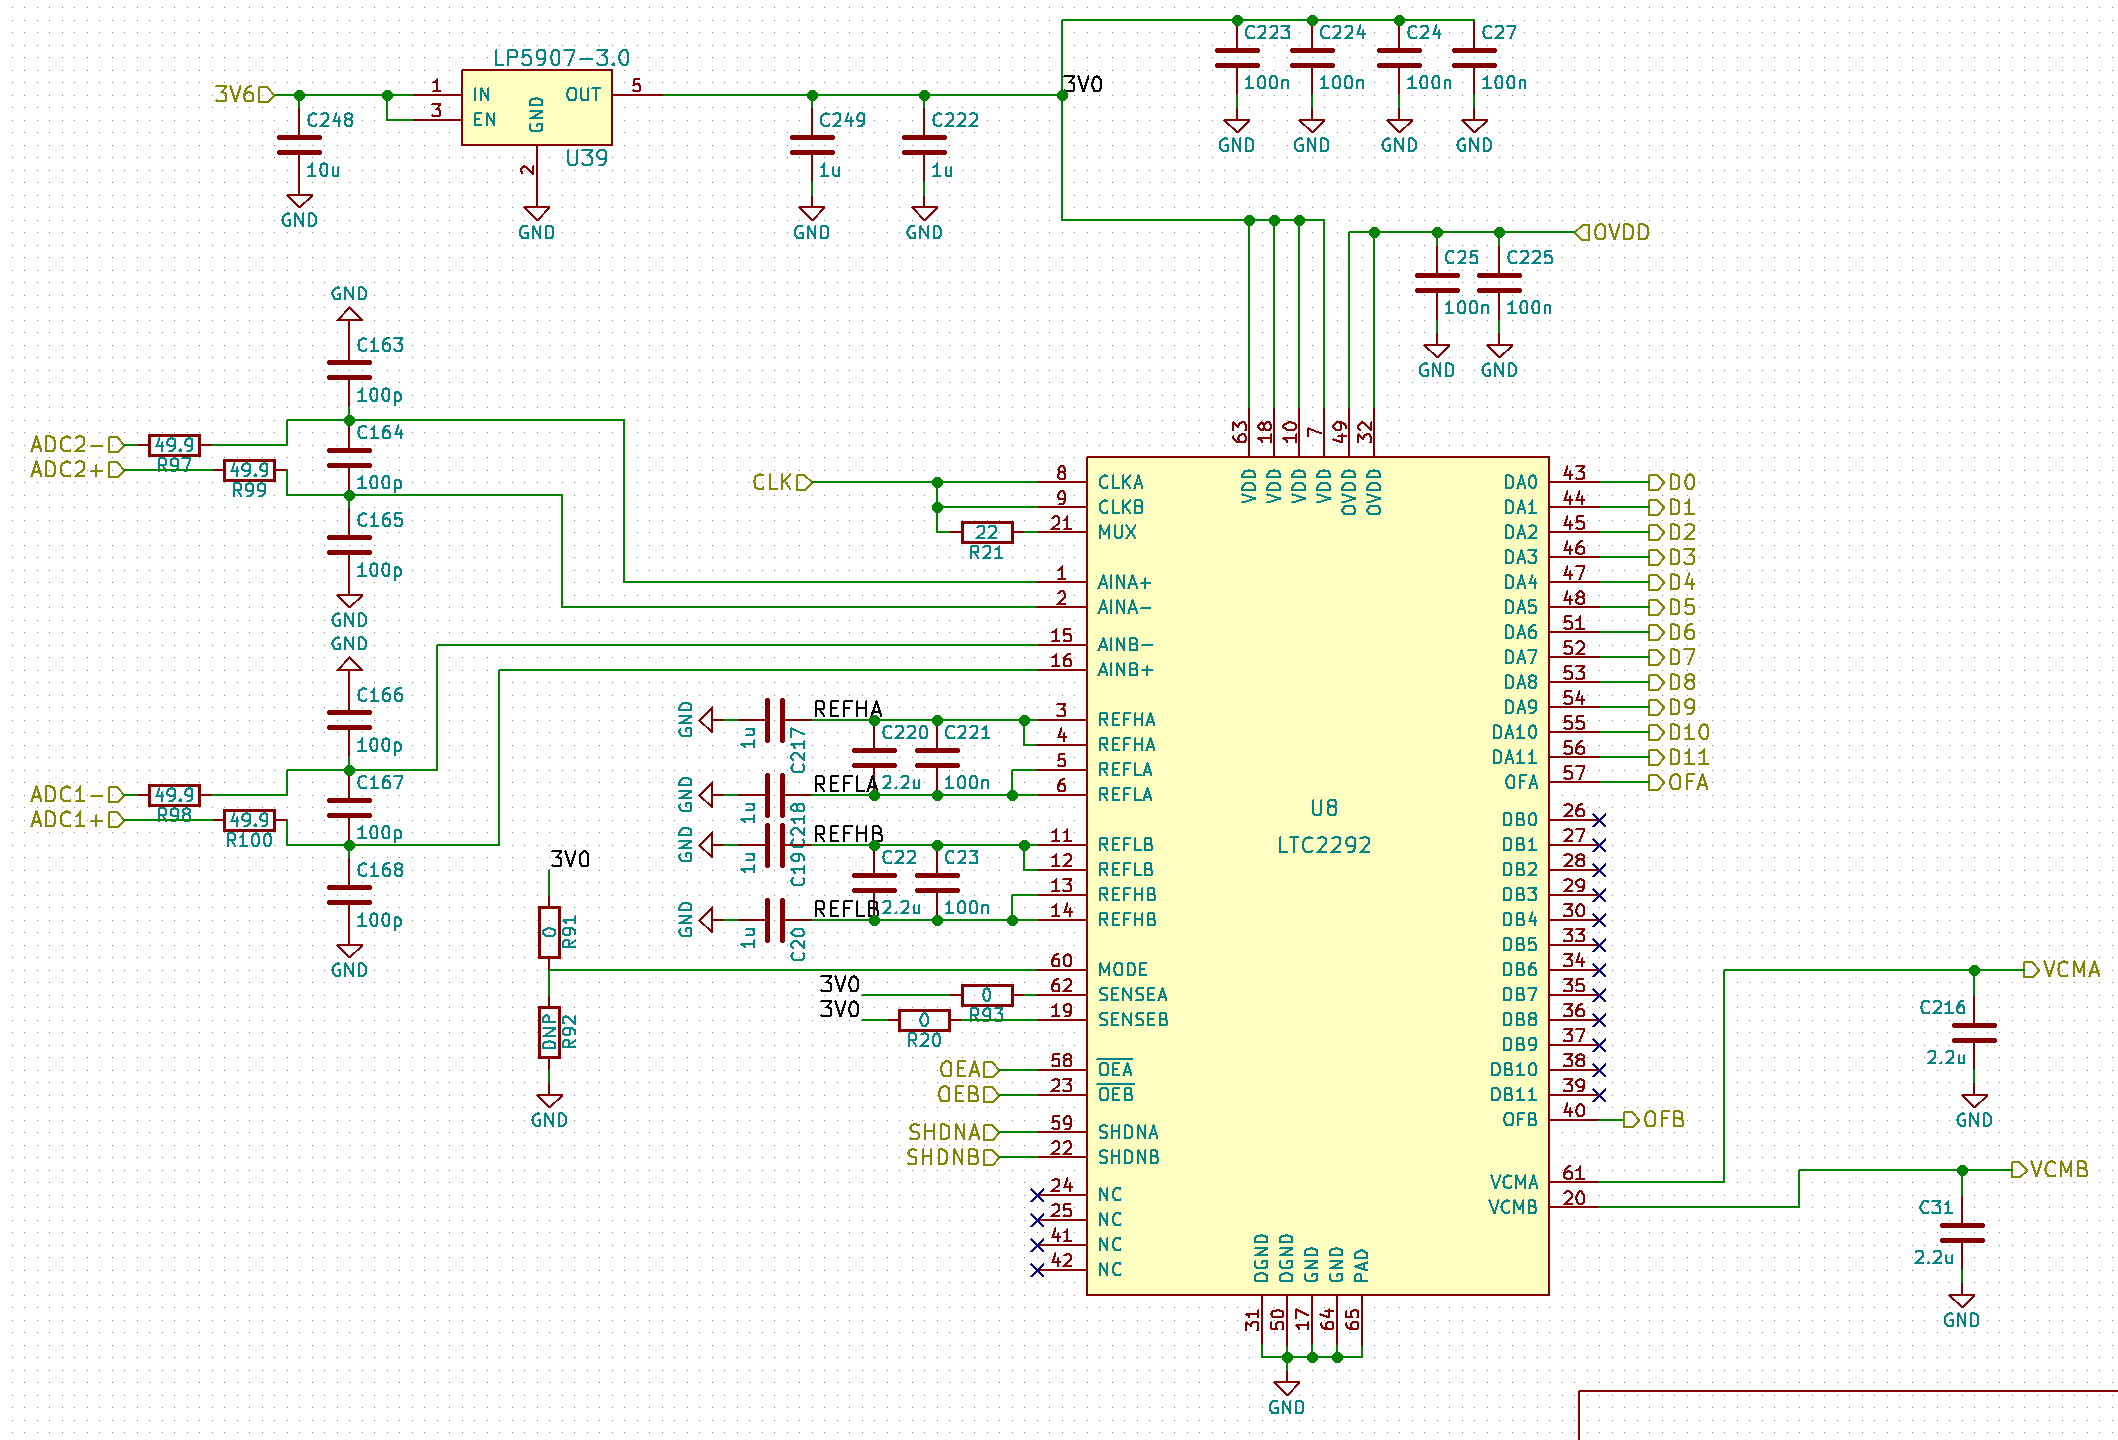
\includegraphics[width=\textwidth]{data/ltc2292-schematic.png}
  \caption{The LTC2292ADC schematic.}
  \label{fig:ltc2292-schematic}
\end{figure}

\begin{figure}[h]
  \centering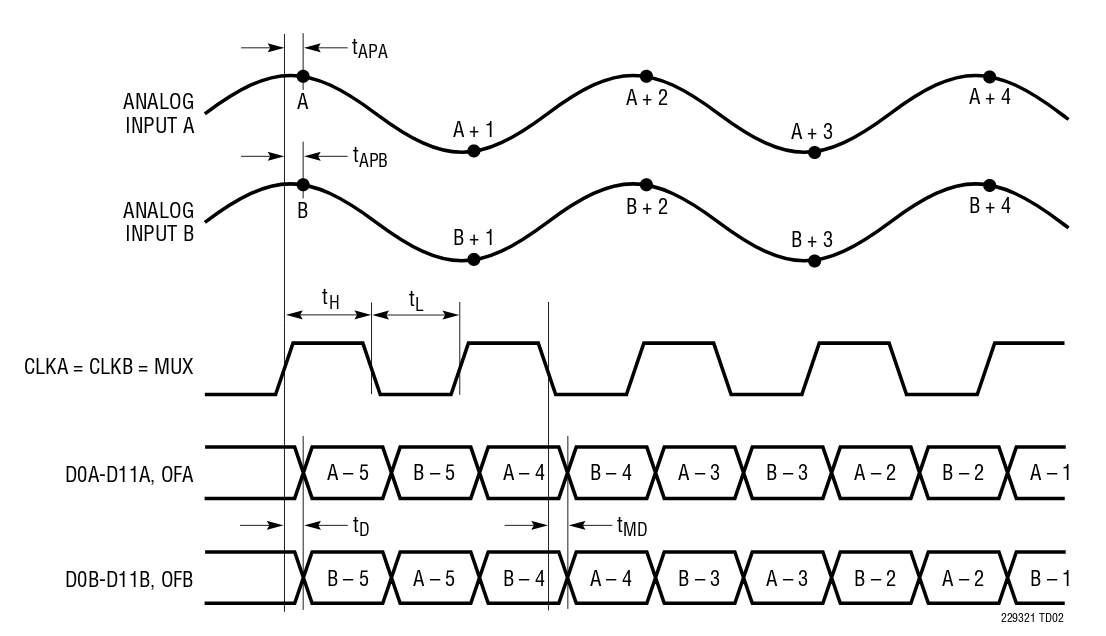
\includegraphics[width=0.75\textwidth]{data/LTC2292-multiplex.png}
  \caption{Multiplexed digital output bus timing for the LTC2292 ADC.}
  \label{fig:ltc2292-multiplex}
\end{figure}

\label{tab:ltc2292-pinout}
\begin{tabularx}{\textwidth}{>{\hsize=.25\hsize} X >{\hsize=.25\hsize} XX}
  \caption{All LTC2292 ADC pin connections in logical groupings.} \\
  \toprule\textbf{LABELS} & \textbf{PIN \#s} & \textbf{DESCRIPTION} \\
  \midrule
  \endhead

  VDD & 7, 10, 18, 63 & The power supply required is 3.0V and each pin requires its own 0.1$\mu$F
                        capacitor. When designing the PCB, ensure that each capacitor is placed as close to its
                        corresponding pin as possible to minimize the trace inductance. The 3.0V signal itself
                        is generated by using an LP5907 LDO regulator that takes in a 3.6V signal.\\
  OVDD & 39, 42 & The power supply for the output that the ADC feeds to, which is the FPGA and takes
                  a 3.3V power supply. So, we connect this to the 3.3V power rail and bypass it with
                  two 0.1$\mu$F capacitors, one for each pin. Again, each should be placed adjacent
                  to their corresponding pins (39 and 42). \\
  CLKA, CLKB, MUX & 8, 9, 21 & Feeds a 40MHz clock signal to the device and specifies that the
                               digitized channel A and B data should be multiplexed and pass through
                               both output buses A and B. We leave B unconnected, so only bus A
                               matters. \\
  DA0-DA11 & 43-48, 51-56 & The digitized output data that contains the input data from both
                            channels A and B, multiplexed. This is fed into the FPGA for
                            processing. \\
  OFA & 57 & This pin is driven high when overflow or underflow occurs. Otherwise it is kept low. We
             export this to the FPGA, although it is not currently used by the FPGA logic. \\
  DB0-DB11 & 26-30, 33-39 & The channel B data bus. Since we multiplex everything through the
                            channel A data bus, this data bus is redundant and therefore left unconnected. \\
  OFB & 40 & Similar to OFA, but for channel B. This is exported to the FPGA, but is also unused. \\
  VCMA, VCMB & 61, 20 & A 1.5V signal that is used to set the common-mode voltage of the IF
                        differential amplifiers, whose outputs are sent to this ADC. They are each
                        bypassed to GND with a 2.2$\mu$F capacitor, which should be placed directly
                        next to their respective pins. \\
  GND, OGND & 17, 64, 65, 31, 50 & The ADC power ground and output power ground, respectively. These
                                   can all be routed to the same ground plane. \\
  NC & 24-25, 41-42 & No connect. \\
  SHDNA, SHDNB, OEA, OEB & 59, 22, 58, 23 & These are input pins that are connected to the FPGA. The
                                            FPGA logic can ground both SHDNA and OEA to allow
                                            channel A to operate normally or bring them both high to
                                            put channel A in sleep mode. Channel B works the same
                                            way. \\
  SENSEA, SENSEB & 62, 19 & These are connected to VDD, which specifies that the input voltage range
                            of the differential signals for both channels A and B is 1.5V $\pm$
                            1V. 1.5V is the common-mode voltage and the channels allow a 2V range
                            around that. \\
  MODE & 60 & Connecting mode to VDD specifies the output format as 2s complement and turns of the
              clock duty stabilizer, which is unnecessary because the input clock has a 50\% duty
              cycle. \\
  REFHA, REFLA, REFLB, REFHB & 3-6, 11-14 & These are the high and low reference for channels A and
                                            B, respectively. Their connection is specified exactly
                                            by the datasheet. It is critical that the 0.1$\mu$F
                                            capacitor is placed as close to the pins as possible. \\
  AINA+, AINA-, AINB-, AINB+ & 1-2, 15-16 & The positive and negative differential inputs for
                                            channels A and B. \textbf{\{STARTINCOMPLETE\}} These
                                            lines have a capacitor between the positive and negative
                                            analog inputs, as well as capacitors connecting each
                                            line to GND. The capacitor value between the lines of
                                            0.1$\mu$F is different from the suggested value of 12pF
                                            and the capacitors connecting the lines to GND are not
                                            suggested from the datasheet (see page 18 of the
                                            datasheet). Additionally, the resistance value of
                                            49.9$\Omega$ differs from the suggested resistance of
                                            25$\Omega$. Lastly, the negative output of the
                                            differential amplifier for channel A is feeding into the
                                            positive input line \textbf{\{END INCOMPLETE\}}. \\

  \bottomrule
\end{tabularx}